\section{Graphics}


\slide{Full-slide image}
{
\insImgCenter{0.25}{pic/transistor}
\sourceRefUrl{https://upload.wikimedia.org/wikipedia/commons/e/e2/Transistor-die-KSY34.jpg} % image source (creative common license)
}


\slide{Image with source-reference link shifted}
{
\insImg{-0.30}{0.12}{0.31}{pic/transistor}
\insImg{0.50}{0.12}{0.25}{pic/transistor}
\vspace{15em}
\sourceRefUrlShifted{50em}{https://upload.wikimedia.org/wikipedia/commons/e/e2/Transistor-die-KSY34.jpg} % image source
}


\slide{Box around image part}
{
\begin{center}
\begin{tikzpicture}
\node[anchor=south west, inner sep=0] at (0,0) { 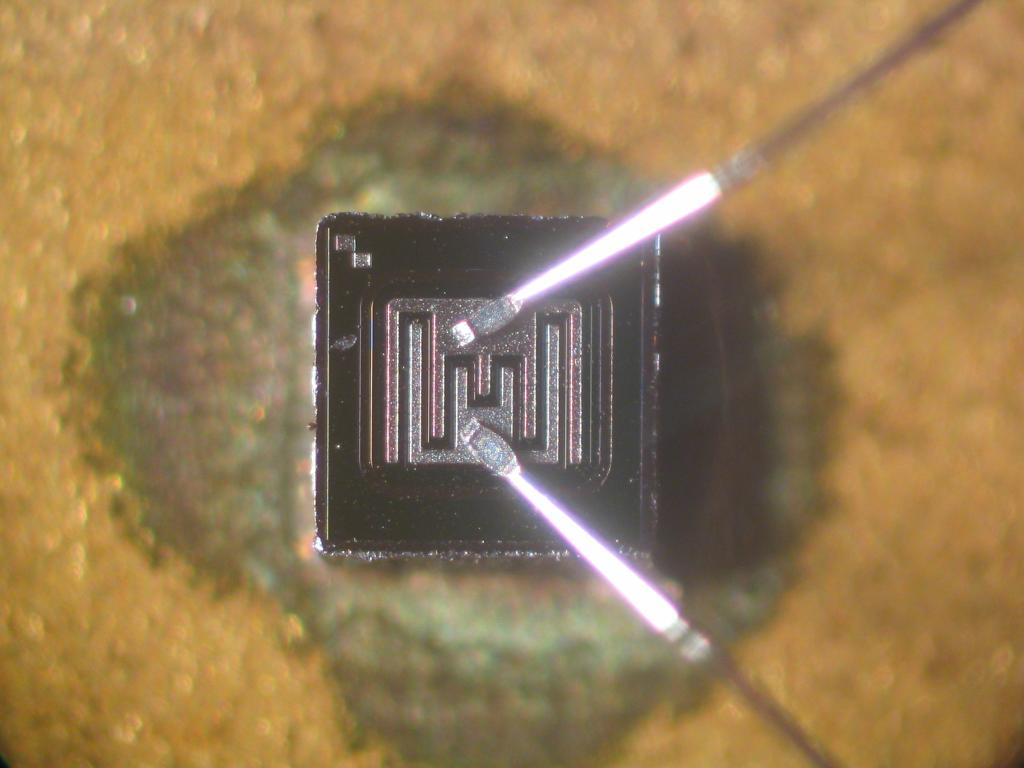
\includegraphics[scale=0.25]{pic/transistor} };
\draw<1>[green,thick,       rounded corners] (2.7, 1.6) rectangle (\textheight-3.2cm, 5);
\draw<2>[red,  ultra thick, rounded corners] (3.9, 2.5) rectangle (4.8, 3.2);
\end{tikzpicture}
\end{center}
\sourceRefUrl{https://upload.wikimedia.org/wikipedia/commons/e/e2/Transistor-die-KSY34.jpg} % image source (creative common license)
}


\slide{Images on the same page}
{
\begin{center}
\includegraphics<1>[scale=0.125]{pic/transistor}
\pause
\includegraphics<2>[scale=0.25]{pic/transistor}
\end{center}
\sourceRefUrl{https://upload.wikimedia.org/wikipedia/commons/e/e2/Transistor-die-KSY34.jpg} % image source (creative common license)
}


\slide{Image decorations}
{
\begin{itemize}
\item Lorem ipsum dolor sit amet,
\item consectetur adipisicing elit,
\item sed do eiusmod tempor incididunt
\item ut labore et dolore magna aliqua.
\item Ut enim ad minim veniam, quis
\item nostrud exercitation ullamco laboris
\item nisi ut aliquip ex ea commodo consequat.
\item Duis aute irure dolor in reprehenderit
\item in voluptate velit esse cillum dolore
\item eu fugiat nulla pariatur.
\end{itemize}
\insImg{0.8}{0.2}{0.05}{pic/transistor}
\pause

\insImgFr{2-}{0.8}{0.55}{0.08}{pic/transistor}
}


\slide{Images interleaved with text}
{
Lorem ipsum dolor sit amet, consectetur adipisicing elit, sed do eiusmod tempor incididunt ut labore et dolore magna aliqua.

\begin{center}
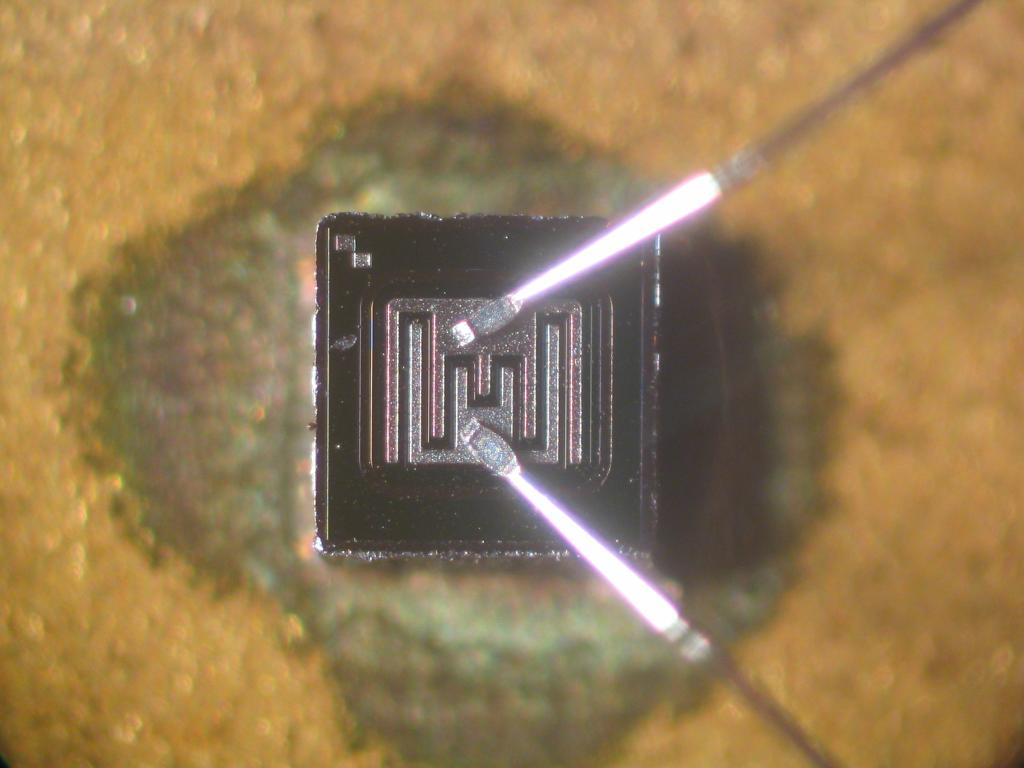
\includegraphics[scale=0.1]{pic/transistor}
\end{center}

Ut enim ad minim veniam, quis nostrud exercitation ullamco laboris nisi ut aliquip ex ea commodo consequat.
}


\slide{PNGs out of SVGs}
{
\begin{center}

\includegraphics[scale=0.5]{svg/biohazard}
\end{center}
}


\slide{} % unnamed!
{
\begin{center}
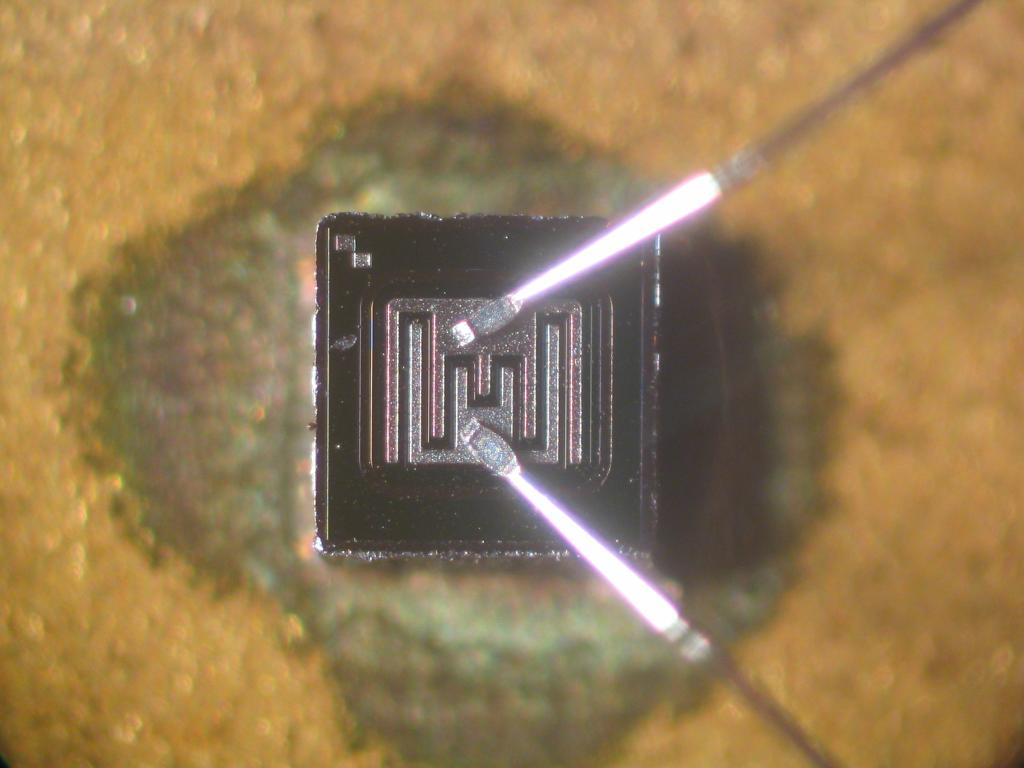
\includegraphics[scale=0.33]{pic/transistor}
\end{center}
}


\slide{Keeping space for images}
{
\begin{block}{Note}
Thanks to usage of \texttt{onslide} image sizes are preserved, even if not displayed.
Reserving space means things do not float between slide changes.
\end{block}

\begin{columns}

\begin{column}{0.33\textwidth}
\begin{center}
Column 1
\end{center}
\end{column}

\begin{column}{0.33\textwidth}
\begin{center}
Column 2
\end{center}
\end{column}

\begin{column}{0.33\textwidth}
\begin{center}
Column 3
\end{center}
\end{column}

\end{columns}

\begin{columns}

\begin{column}{0.33\textwidth}
\begin{center}
\onslide<2->{ \insImgCenter{0.1}{pic/transistor} }
\end{center}
\end{column}

\begin{column}{0.33\textwidth}
\begin{center}
\onslide<3->{ \insImgCenter{0.2}{svg/biohazard} }
\end{center}
\end{column}

\begin{column}{0.33\textwidth}
\begin{center}
\onslide<4->{ \insImgCenter{0.6}{pic/plantuml_logo} }
\end{center}
\end{column}

\end{columns}
}
